%%!TEX encoding = UTF-8 Unicode

% According to UA rules, font size should range from 10 to 12pt.
\documentclass[11pt,a4paper,openright,final,twoside,onecolumn]{memoir}

\listfiles
\fixpdflayout

\usepackage[utf8]{inputenc}

% Computer Modern Typewritter (For bold ttfamily in listings)
\usepackage{lmodern}
% OR... Bera Mono
%\usepackage[scaled]{beramono} % TTT Font
%\usepackage{anyfontsize} % As the name says...

\usepackage[T1]{fontenc}

% For Overleaf support
\usepackage{ifthen}
\def\useoverleaf{0}  % change to non-zero (for instance, 1) to enable it

\makeatletter
\newcommand{\makecoverfile}[0]{%
  \immediate\write18{latexmk -pdf cover.tex}%
}
\makeatother

%For PDF merging
\usepackage{pdfpages}

%SET DPI to 300
\pdfpxdimen=\dimexpr 1in/300\relax

\usepackage{morewrites} % Allow the use of a larger number of packages

%For English and Portuguese languages
%Portuguese will be the default.
%Use \setdefaultlanguage to change it
\usepackage{csquotes}
\usepackage[english]{babel}

% For custom date format
\usepackage{datetime}
\newdateformat{thesisdate}{\monthname[\THEMONTH] \THEYEAR} % Month Year

\usepackage{microtype} % Make pdf look better


% Uncomment to enable floats on facing pages
%\usepackage{dpfloat}

%Side by side figures
% Eg. Fig 1a, Fig 1b
\usepackage[hang,small,bf]{caption}
%\let\tion\undefined
%\let\subfloat\undefined
\usepackage{subcaption}

%\RequirePackage{textcase}

% Dropped Caps
%\usepackage{lettrine}


% Configure Hyperlink color
%\usepackage[breaklinks=true,colorlinks=false,linkcolor=blue]{hyperref}
% Or use the default
\usepackage{hyperref}

%Optional: Redefine section names
%\def\sectionautorefname{Section}
%\def\chapterautorefname{Chapter}
%\def\figureautorefname{Figure}
%\def\listingautorefname{Listing}
%\def\tableautorefname{Table}

%For PDF Comments
\usepackage{comment}
\usepackage{pdfcomment}
\usepackage{bookmark} % New Bookmarks

%For Multiple columns in Glossary
%\usepackage{multicol}
\usepackage[nonumberlist,acronym]{glossaries}
\renewcommand{\glossarysection}[2][]{}  % So it doesn't print glossary package titles
\makeglossaries

%Math symbols
\usepackage{amsmath}
\usepackage{amssymb}

%Text symbols
\usepackage{pifont}
\newcommand{\cmark}{\ding{51}}
\newcommand{\xmark}{\ding{55}}

%Graphics
\usepackage{graphicx}

%Colors
\usepackage{xcolor}

%Euro symbol
\usepackage{eurosym}

% Code boxes
\ifthenelse{\equal{\useoverleaf}{0}}
{\usepackage[outputdir=build]{minted}}
{\usepackage{minted}}%

\renewcommand\listingscaption{Código}
\fvset{fontsize=\footnotesize} % Make Code blocks smaller than text

%Biber using IEEE style for proper UTF-8 support
\usepackage[backend=biber,style=ieee, sorting=none]{biblatex}
\bibliography{bib/references.bib, bib/rfc.bib}

%Use acronyms
\usepackage[printonlyused]{acronym} % For acronyms

% Enable chart support through pgf and tikz
\usepackage[version=0.96]{pgf}
\usepackage{tikz}
\usepackage{pgf-umlsd}
\usetikzlibrary{arrows,shadows,trees,shapes,snakes,automata,backgrounds,petri,mindmap} % for pgf-umlsd

% For inline TT text (e.g. code snippets)
\usepackage{verbatim}

 %Frames around figures and allow force placement
\usepackage{float}

\usepackage{makecell}

%Configure Float style
%\floatstyle{boxed}
%\restylefloat{table}
%\restylefloat{figure}
%\restylefloat{lstlisting}

%Keep floats inside section!
\usepackage[section]{placeins}
\let \oldsubsubsection \subsubsection
\renewcommand{\subsubsection}[2][]{
  \FloatBarrier
  \oldsubsubsection#1{#2}
}
\let \oldsubsection \subsection
\renewcommand{\subsection}[2][]{
  \FloatBarrier
  \oldsubsection#1{#2}
}
\let \oldsection \section
\renewcommand{\section}[2][]{
  \FloatBarrier
  \oldsection#1{#2}
}
\let \oldchapter \chapter
\renewcommand{\chapter}[2][]{
  \FloatBarrier
  \oldchapter#1{#2}
}


%%%% Use the built-in division styling
\headstyles{memman}

%%% ToC down to subsections
\settocdepth{subsection}

%%% Numbering down to subsections as well
\setsecnumdepth{subsection}

%%%% extra index for first lines
\makeindex[lines]

%Margins for University of Aveiro Thesis
\setlrmarginsandblock{3cm}{2.5cm}{*}
\setulmarginsandblock{3cm}{3cm}{*}
\checkandfixthelayout

%Or custom spacing
%\addtolength{\parskip}{0.5\baselineskip}
\linespread{1.5}

\begin{document}
%\ifthenelse{\equal{\useoverleaf}{0}}{}{\makecoverfile{}}%
%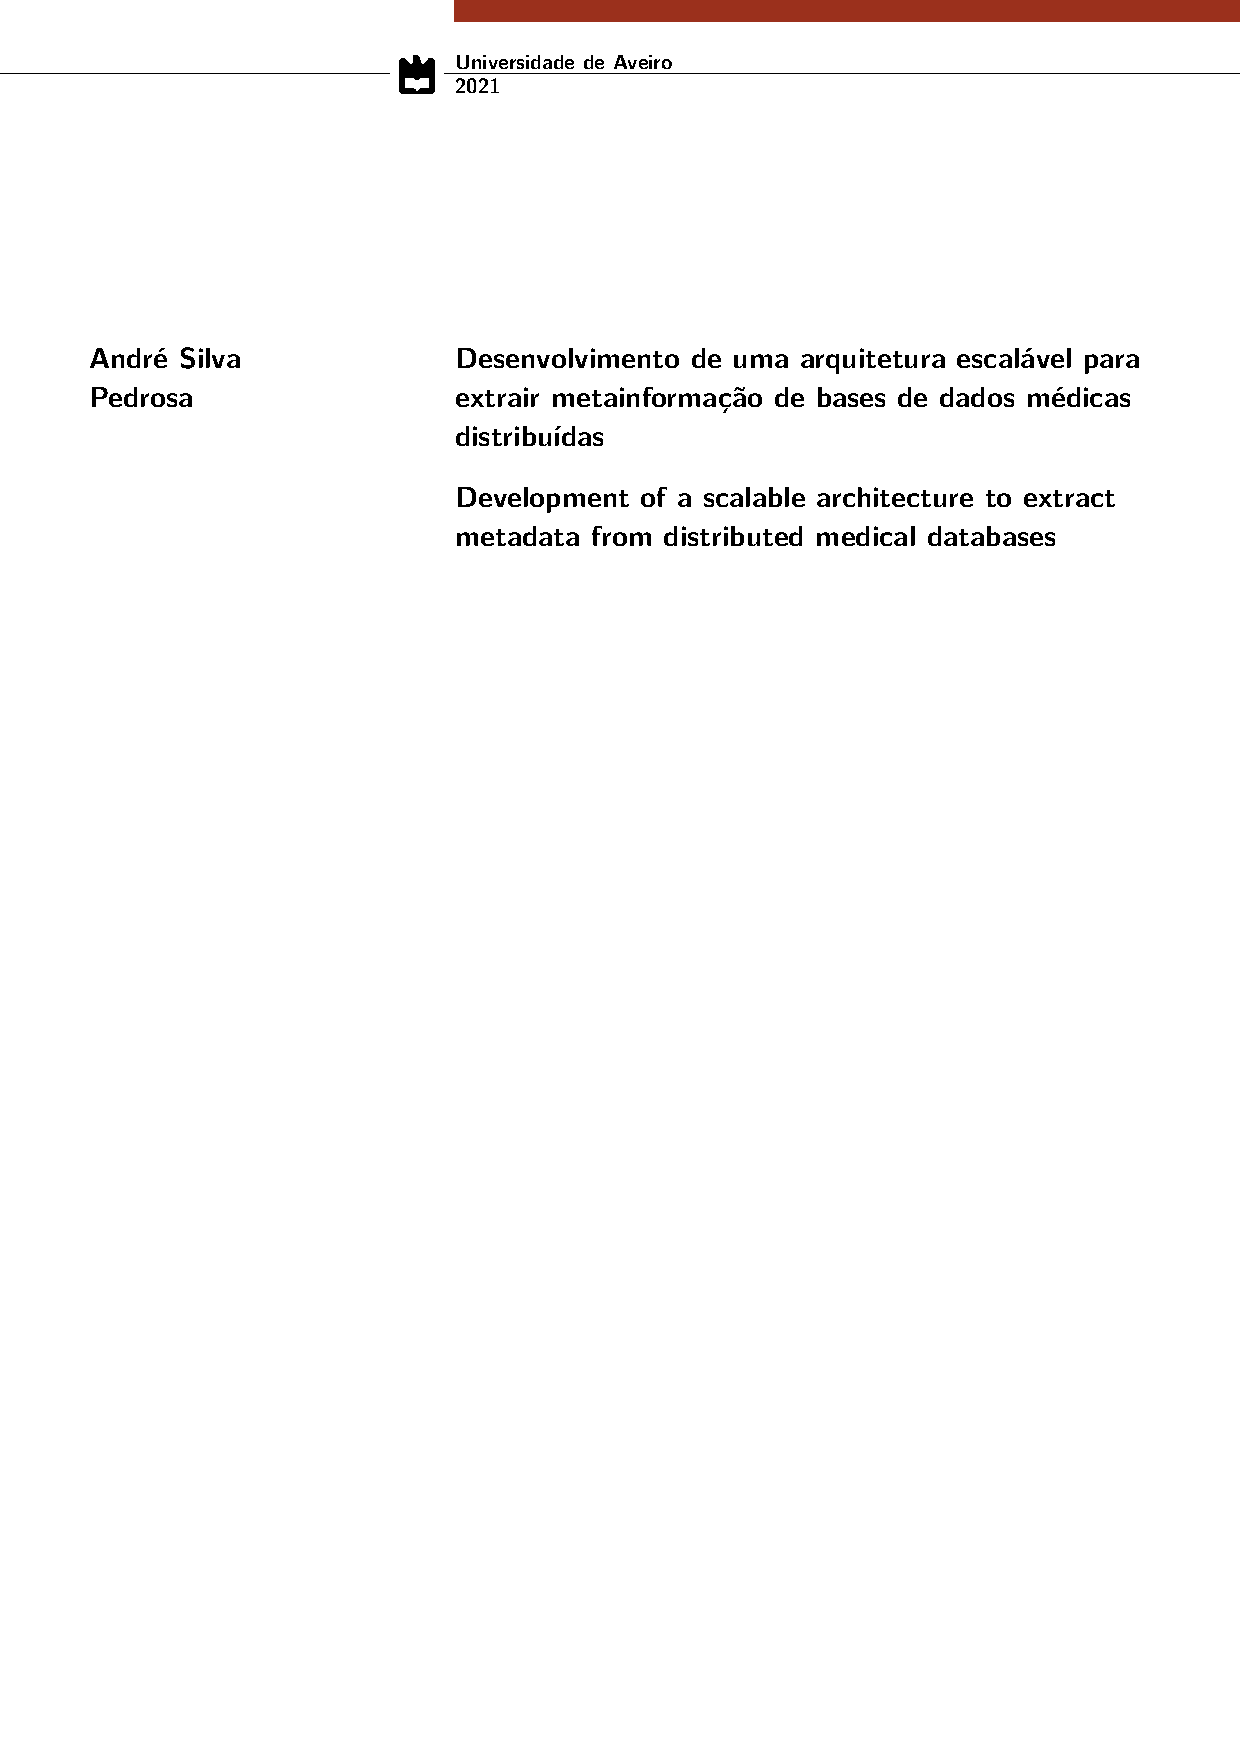
\includepdf[pages=-]{cover.pdf}

%
%Front matter

%Custom Chapter style named thesis
\makechapterstyle{thesis}{% Based on ell
  \chapterstyle{default}
  \renewcommand*{\chapnumfont}{\normalfont\sffamily}
  \renewcommand*{\chaptitlefont}{\normalfont\Huge\sffamily}
  \settowidth{\chapindent}{\chapnumfont 111}
  \renewcommand*{\chapterheadstart}{\begingroup
    \vspace*{\beforechapskip}%
    \begin{adjustwidth}{}{-\chapindent}%
    \hrulefill
    \smash{\rule{0.4pt}{15mm}}
    \end{adjustwidth}\endgroup}
  \renewcommand*{\printchaptername}{}
  \renewcommand*{\chapternamenum}{}
  \renewcommand*{\printchapternum}{%
    \begin{adjustwidth}{}{-\chapindent}
    \hfill
    \raisebox{10mm}[0pt][0pt]{\fontsize{30}{25}\selectfont\chapnumfont \thechapter}%
                              \hspace*{1em}
    \end{adjustwidth}\vspace*{-3.0\onelineskip}}
  \renewcommand*{\printchaptertitle}[1]{%
    \vskip\onelineskip
    \raggedleft {\chaptitlefont ##1}\par\nobreak\vskip 4\onelineskip}}


%Select chapter style from existing or select custom
%\chapterstyle{thesis} % Others: dowding, demo2, dash, chappell, brotherton, bianchi, ger, madsen, tatcher, veelo,indexes)
% thesis can also be used as defined previously
%

%If you feel adventurous you can also define all aspects of your theme
%Use either this input or the chapterstyle before
%% Rules
\newcommand{\thinRule}{\rule{\textwidth}{0.25pt}}

% Customize heading appearances
% Define styles
\newcommand{\partSize}{\Huge}
\newcommand{\partStyle}{\lsstyle\scshape}
\newcommand{\chapterSize}{\Huge}
\newcommand{\chapterStyle}{\lsstyle\scshape}
\newcommand{\chapterAfter}{}
\newcommand{\sectionSize}{\Large}
\newcommand{\sectionStyle}{\scshape\MakeTextLowercase}
\newcommand{\subsectionSize}{\large}
\newcommand{\subsectionStyle}{\scshape\MakeTextLowercase}
\newcommand{\subsubsectionSize}{\large}
\newcommand{\subsubsectionStyle}{\scshape\MakeTextLowercase}
\newlength{\partNumSizePt}
\setlength{\partNumSizePt}{60pt}
\newlength{\chapterNumSizePt}
\setlength{\chapterNumSizePt}{60pt}
\newcommand{\partNumSize}{%
  \fontsize{\partNumSizePt}{1.2\partNumSizePt}\selectfont%
}
\newcommand{\partNumStyle}{\partChapterNumColor}
\newcommand{\chapterNumSize}{%
  \fontsize{\chapterNumSizePt}{1.2\chapterNumSizePt}\selectfont%
}
\newcommand{\chapterNumStyle}{\partChapterNumColor}

% Customize parts
\renewcommand{\partnamefont}{\partSize\partStyle}
\renewcommand{\partnumfont}{\partNumSize\partNumStyle}
\renewcommand{\printpartname}{}
\renewcommand{\printparttitle}[1]{%
  \normalfont\normalcolor\partnamefont #1
}

% Customize chapters
\makeatletter
\setlength{\beforechapskip}{30pt}
\renewcommand*{\chapterheadstart}{\vspace*{\beforechapskip}}
\setlength{\afterchapskip}{3ex}
\setlength{\midchapskip}{3ex}
\renewcommand*{\chapnamefont}{%
  \Large\flushright\chapterStyle\partChapterNumColor%
}
\renewcommand*{\chapnumfont}{\chapterNumSize\chapterNumStyle}
\renewcommand*{\chaptitlefont}{%
  \normalfont\flushleft\normalcolor\chapterSize\chapterStyle%
}
\renewcommand*{\printchaptername}{%
  \chapnamefont\MakeTextLowercase{\@chapapp}%
}
\renewcommand*{\chapternamenum}{\quad}
\renewcommand*{\printchapternum}{%
%  \chapnumfont\textls[-75]{\classicstylenums{\thechapter}}%
 \chapnumfont\textls[-75]{\thechapter}%

}
\renewcommand*{\printchaptertitle}[1]{%
  \chaptitlefont #1
  \chapterAfter
}
\makeatother
% Customize sections and subsections
\setsecnumformat{\csname my#1\endcsname\quad}
\setsecheadstyle{\sectionSize\sectionStyle}
\newcommand{\mysection}{{\thesection}}
\setlength{\beforesecskip}{3em}


\setsubsecheadstyle{\subsectionSize\subsectionStyle}
\newcommand{\mysubsection}{{\normalfont\subsectionSize\thesubsection}}
\setlength{\beforesubsecskip}{3em}

\setsubsubsecheadstyle{\subsubsectionSize\subsubsectionStyle}
\newcommand{\mysubsubsection}{{\normalfont\subsubsectionSize\thesubsubsection}}
\setlength{\beforesubsubsecskip}{2em}

% Customize "Table of ..." appearance
% Customize headings
\newcommand{\renewPrintXTitle}[1]{%
  \renewcommand{#1}[1]{%
    \printchaptertitle{##1}%
  }%
}
\renewPrintXTitle{\printtoctitle}
\renewPrintXTitle{\printlottitle}
\renewPrintXTitle{\printloftitle}

% Customize ToC headings
\renewcommand{\cftpartfont}{\partChapterNumColor\partStyle}
\renewcommand{\cftchapterfont}{\chapterStyle}
\renewcommand{\cftsectionfont}{}
\renewcommand{\cftsubsectionfont}{}
\renewcommand{\cftfigurefont}{}
\renewcommand{\cfttablefont}{}
\newcommand{\cftlstlistingfont}{}

% Increase number width
\newlength{\cftNumWidthIncrease}
\setlength{\cftNumWidthIncrease}{0.25em}
\addtolength{\cftpartnumwidth}{\cftNumWidthIncrease}
\addtolength{\cftchapternumwidth}{\cftNumWidthIncrease}
\addtolength{\cftsectionindent}{\cftNumWidthIncrease}
\addtolength{\cftsubsectionindent}{\cftNumWidthIncrease}
% No leader dots
%\renewcommand*{\cftpartdotsep}{\cftnodots}
%\renewcommand*{\cftchapterdotsep}{\cftnodots}
%\renewcommand*{\cftsectiondotsep}{\cftnodots}
%\renewcommand*{\cftsubsectiondotsep}{\cftnodots}
%\renewcommand*{\cftfiguredotsep}{\cftnodots}
%\renewcommand*{\cfttabledotsep}{\cftnodots}
%\newcommand*{\cftlstlistingdotsep}{\cftnodots}
% Set page numbers immediately after entry text
\newcommand{\tocEntryPageSep}{\hspace{1em}}
\renewcommand{\cftpartleader}{\cftdotfill{\cftdotsep}}
%\renewcommand{\cftpartafterpnum}{\cftparfillskip}
%\renewcommand{\cftchapterleader}{\tocEntryPageSep}
\renewcommand{\cftchapterleader}{\cftdotfill{\cftdotsep}}
%\renewcommand{\cftchapterafterpnum}{\cftparfillskip}
\renewcommand{\cftsectionleader}{\cftdotfill{\cftdotsep}}
%\renewcommand{\cftsectionafterpnum}{\cftparfillskip}
\renewcommand{\cftsubsectionleader}{\cftdotfill{\cftdotsep}}
%\renewcommand{\cftsubsectionafterpnum}{\cftparfillskip}
\renewcommand{\cftfigureleader}{\cftdotfill{\cftdotsep}}
%\renewcommand{\cftfigureafterpnum}{\cftparfillskip}
\renewcommand{\cfttableleader}{\cftdotfill{\cftdotsep}}
%\renewcommand{\cfttableafterpnum}{\cftparfillskip}
\newcommand{\cftlstlistingleader}{\cftdotfill{\cftdotsep}}
%\newcommand{\cftlstlistingafterpnum}{\cftparfillskip}
% Customize page numbers
\newcommand{\tocPageStyle}{\tocPageColor}
\renewcommand{\cftpartpagefont}{\tocPageStyle}
\renewcommand{\cftchapterpagefont}{\tocPageStyle}
\renewcommand{\cftsectionpagefont}{\tocPageStyle}
\renewcommand{\cftsubsectionpagefont}{\tocPageStyle}
\renewcommand{\cftfigurepagefont}{\tocPageStyle}
\renewcommand{\cfttablepagefont}{\tocPageStyle}
\newcommand{\cftlstlistingpagefont}{\tocPageStyle}

% Abstract
% Remove indents around abstract text
\setlength{\absleftindent}{0pt}
\setlength{\absrightindent}{0pt}
% Change font size to conform with the rest of the document text
\renewcommand{\abstracttextfont}{\normalsize}

% Customize headers and footers including page numbers
\newcommand{\hfTextSize}{\footnotesize}
\newcommand{\headTextStyle}{\lsstyle\scshape\MakeTextLowercase}
\nouppercaseheads
\makeevenhead{headings}%
             {\hfTextSize\thepage}%
             {}%
             {\hfTextSize\headTextStyle\leftmark}
\makeevenhead{plain}%
             {\hfTextSize\thepage}%
             {}%
             {\hfTextSize\headTextStyle\leftmark}
\makeoddhead{headings}%
            {\hfTextSize\headTextStyle\rightmark}%
            {}%
            {\hfTextSize\thepage}
\makeoddhead{plain}%
            {\hfTextSize\headTextStyle\rightmark}%
            {}%
            {\hfTextSize\thepage}


% Customize captions
\newcommand{\captionSize}{\small}
\newcommand{\captionStyle}{\scshape}
\newcommand{\captionWidthRatio}{0.9}

\captionnamefont{\captionSize\captionStyle}
\captiontitlefont{\captionSize}
\captiondelim{ -- }
\captiontitlefinal{}
\changecaptionwidth
%\captionwidth{\captionWidthRatio\textwidth}

% Define colors
%\newcommand{\titleColor}{\color[rgb]{0.616, 0.0627, 0.176}}
\newcommand{\titleColor}{\color[rgb]{0,0,0}}

\newcommand{\partChapterNumColor}{\titleColor}
\newcommand{\dropCapColor}{\titleColor}
%\newcommand{\tocPageColor}{\color[rgb]{0.0980, 0.329, 0.651}}

\newcommand{\tocPageColor}{\color[rgb]{0, 0,0}}
\definecolor{shade0}{rgb}{1.0 , 1.0 , 1.0 }
\definecolor{shade1}{rgb}{0.9 , 0.9 , 0.9 }
\definecolor{shade2}{rgb}{0.8 , 0.8 , 0.8 }
\definecolor{shade3}{rgb}{0.65, 0.65, 0.65}
\definecolor{shade4}{rgb}{0.45, 0.45, 0.45}
\definecolor{shade5}{rgb}{0.0 , 0.0 , 0.0 }



\chapterstyle{veelo}
%Exclude sub figures from List of Figures
%\captionsetup[subfloat]{list=no}


% Texts
\newenvironment{introduction}
{%
  \begin{minipage}{\textwidth}%
   \itshape%
}
{%
  \end{minipage}%
  \par\addvspace{2\baselineskip plus 0.2\baselineskip minus 0.2\baselineskip}%
}


%Select Page style
\pagestyle{plain}

\frontmatter

\tightlists
\midsloppy
\raggedbottom

\setcounter{tocdepth}{2} %subsections are added to the TOC
\setcounter{secnumdepth}{4} %subsubsections are numbered


\cleardoublepage

%Table of contents
%%{\small\tableofcontents}
%%\cleardoublepage

%List of figures
%{\small\listoffigures}


%List of tables
%%\cleardoublepage
%%{\small\listoftables}

%Print Glossary
{\small \newacronym{ehden}{EHDEN}{European Health Data and Evidence Network}
\newacronym{ohdsi}{OHDSI}{Observational Health Data Sciences and Informatics}
\newacronym{eu}{EU}{European Union}
\newacronym{cdm}{CDM}{Common Data Model}
\newacronym{omop}{OMOP}{Observational Medical Outcomes Partnership}
\newacronym{fair}{FAIR}{Findability, Accessibility, Interoperability, and Reusability}
\newacronym{api}{API}{Application Programmable Interface}
\newacronym{redcap}{REDCap}{Research Electronic Data Capture}
\newacronym{gaain}{GAAIN}{Global Alzheimer's Association Interactive Network}
\newacronym{dpc}{DPC}{Data Partner Clients}
\newacronym{bbmri-eric}{BBMRI-ERIC}{Biobanking and BioMolecular Resources Research Infrastructure-European Research
Infrastructure Consortium}
\newacronym{rd}{RD}{Research and Development}
\newacronym{achilles}{ACHILLES}{Automated Characterization of Health Information at Large-scale Longitudinal Evidence Systems}
\newacronym{emif}{EMIF}{European Medical Information Framework}
\newacronym{pds}{PDS}{Project Data Sphere}
\newacronym{nada}{NADA}{National Data Archive}
\newacronym{json}{JSON}{JavaScript Object Notation}
\newacronym{dats}{DATS}{DatA Tag Suite}
\newacronym{ehr}{EHR}{Electronic Health Record}
\newacronym{cdw}{CDW}{Clinical Data Warehouse}
\newacronym{crud}{CRUD}{Create, Read, Update and Delete}
\newacronym{xss}{XSS}{Cross-Site Scripting}
\newacronym{html}{HTML}{HyperText Markup Language}
\newacronym{orm}{ORM}{Object–Relational Mapping}
\newacronym{sql}{SQL}{Structured Query Language}
\newacronym{http}{HTTP}{HyperText Transfer Protocol}
\newacronym{ide}{IDE}{Integrated Development Environment}
\newacronym{cdn}{CDN}{Content Delivery Network}
\newacronym{npm}{NPM}{Node Package Manager}
\newacronym{rest}{REST}{Representational State Transfer}
\newacronym{csv}{CSV}{Comma-separated values}
\newacronym{rdbms}{RDBMS}{Relational Database Management System}
\newacronym{amqp}{AMQP}{Advanced Message Queuing Protocol}
\newacronym{jms}{JMS}{Java Message Service}
}


%
%Main document starts here
%
\mainmatter



% Start of Thesis text ----------------------------------------------------------
%Line spacing: 1.5 pt
\OnehalfSpacing

%\chapter{Introduction}
\label{chapter:introduction}

Oftentimes medical researchers do studies associated with diseases, such as determining the impact of a certain drug or find variables that are characteristic of certain diseases.
To perform such studies and have reliable results, a great amount of data is required.
To obtain that data, these researchers have to contact medical data owners to have access to relevant data that can help improve their analysis and/or findings.

With this procedure emerges several problems for the researcher such as he has to find
institutions willing to share data and the process of contacting the data providers can
be cumbersome.
To aid in this whole process, several data hubs have been developed with the purpose of
making the process of data discovery easier.
One important aspect of such data hubs is that they present to the researcher meta
data, which is aggregations or summaries of the original data.
Metadata has the advantage that one doesn't have to deal with the anonymization process
of medical records, since only summaries of the initial data are retrieved
~\cite{egenvar, montra}.
With this dependency on the original data, emerges an important problem of data hubs
which is, metadata can easily be outdated after a small time window.
This could not raise a big problem, if the records were updated regularly, however this
rarely happens, mainly because either the update process is difficult or because
metadata has to be manually extracted and uploaded to the data hub.
A problem that still might arise from such platforms, is those different datasets very
often have different representation for the same concept or the data is organized in a
different layout.
The research is then hampered since either different approaches have to be taken to
analyze each dataset.

The \gls{ehden}~\cite{ehden} project has affiliations with several institutions, data sources and data custodians across the \gls{eu}, which the main goal is to, within a federated network~\cite{ehden-datapartners}, harmonize their data to the \gls{omop} \gls{cdm}, which was developed by \gls{ohdsi}, a multi-stakeholder, interdisciplinary and collaborative organization that brings out the value of health data through large-scale analytics~\cite{ohdsi-site}.
With a \gls{cdm}, the problem of having different representations for the same data
across distinct data sources is solved.
Researchers can now develop a single analysis method and then apply it to all gathered
datasets and these methods can be optimized for this specific data model, which allows
large-scale analytics.
Furthermore, also improves collaborative research~\cite{ohdsi-site}.
Still, within the scope of the \gls{ehden} project, the project has a database catalog~\cite{ehden-portal},
built with the MONTRA framework~\cite{montra}, where data owners fill metadata about
their data source manually, which brings the outdated problem already mentioned before.
Additionally, whenever new metadata fields are introduced, the data owners of all data
sources have to go manually update their metadata form.

\section{Objectives}
The purpose of this dissertation is to create a system that can automate the update process of metadata stored in online platforms, that aids in the procedure of finding the correct data set for a specific study.
Such a system must be able to extract metadata from the databases, for that, an agent software will be installed along with each databases' local system.
Additionally, as new software components might be developed, it is a great opportunity to try new technologies.

With that, the following goals were established:
\begin{itemize}
    \item have a platform capable of holding and displaying metadata in an intuitive and user-friendly way;
    \item develop or find a tool that extracts metadata from a database;
    \item design a system capable of sending data to an application, to keep their data up-to-date;
    \item make use of new technologies with growing popularity.
\end{itemize}

\section{Outline}
This dissertation is organized into five more chapters, which are described below.

Chapter \ref{chapter:background} intends to provide a state-of-the-art characterization associated with the work of the dissertation.
Regarding the several goals established, several solutions and approaches were studied.

In chapter \ref{chapter:metadata-visualization} a software framework used to develop platforms to store and visualize metadata is described.
Has this framework had some design flaws, the chapter also details all the improvements performed.

Chapter \ref{chapter:extraction-update} describes the entire development process around the tool to extract metadata and the metadata management system that automates the update process of metadata.
It starts by detailing all the requirements associated with such components, then describes both the architecture and implementation of both the extraction tool and the metadata management system.

The Chapter \ref{chapter:evalution} is used to show the integration of all the components developed in the previous chapters.

The last chapter, \ref{chapter:conclusion}, presents the main achievements with the work, main challenges found and future work.

\chapter{Background}
\label{chapter:background}

From a medical standpoint, to perform their studies, researches need to contact data
owners to have access to relevant data that can help improve their analysis and/or
findings that can be applied to real cases.
With this procedure emerges several problems for the researcher such as he has to find
institutions willing to share data and the process of contacting the data providers can
be cumbersome.
To aid in this whole process, several data hubs have been developed with the purpose of
making the process of data discovery easier.
One important aspect of such data hubs is that they present to the researcher meta
data, which is aggregations or summaries of the original data.
Metadata has the advantage that one doesn't have to deal with the anonymization process
of medical records, since only summaries of the initial data are retrieved
\cite{egenvar, montra}.
With this dependency on the original data, emerges an important problem of data hubs
which is, metadata can easily be outdated after a small time window.
This could not raise a big problem, if the records were updated regularly, however this
rarely happens, mainly because either the update process is difficult or because
metadata has to be manually extracted and uploaded to the data hub.
A problem that still might arise from such platforms, is those different datasets very
often have different representation for the same concept or the data is organized in a
different layout.
The research is then hampered since either different approaches have to be taken to
analyze each dataset.

The \gls{ehden} project has affiliations with several institutions, data sources and
data custodians across the \gls{eu}, which the main goal is to, within a federated
network, harmonize their data to the \gls{omop} \gls{cdm}\cite{ehden-datapartners}.
With a \gls{cdm}, the problem of having different representations for the same data
across distinct data sources is solved.
Researchers can now develop a single analysis method and then apply it to all gathered
datasets and these methods can be optimized for this specific data model, which allows
large-scale analytics.
Furthermore, also improves collaborative research \cite{ohdsi-site}.
Still, within the scope of the \gls{ehden} project, the project has a database catalog,
built with the Montra framework \cite{montra}, where data owners fill metadata about
their data source manually, which brings the outdated problem already mentioned before.
Additionally, whenever new metadata fields are introduced, the data owners of all data
sources have to go manually update their metadata form.

To build a valuable data hub is then important to take into account how to:
\begin{itemize}
    \item extract metadata from a data source
    \item upload and update the metadata on the data hub
    \item automatize the two processes mentioned before
    \item receive and display the metadata on the data hub in a way that facilitates
        readability.
\end{itemize}

\section{Metadata visualization tools}
It will then be explored existing visualization platforms that enhance data discovery
by presenting summaries or metadata of records (data sources, datasets).

In some cases data can't be publicly available because it contains sensitive data or
simply the data owner might not want to share some portions of the data, for that the
tools analyzed should have privacy protection mechanisms, allowing to customize the
access and manipulation of data stored.

Furthermore, considering we want to improve and assist data discovery and reuse it is
important to have good data management to simplify such processes.
However, humans fail to achieve the necessary processing levels with present-day
scientific data.
It is then important that data is provided in such a way that machines can fetch,
understand, analyze and act on data.
For that the \gls{fair} Guiding Principles were established which contain a series of
considerations for data publishing to supports both human and machine operations such
as deposition, exploration, sharing and reuse \cite{fair}.

Finally, it is preferential for such a tool to be open source since the available
solution might need some changes to solve our specific problem, and also it makes it
possible to receive contributions from the community.

\subsection{Search Method}

Regarding this subject, there was already done a systematic review of several tools
that fit within the current search pool.
Its objective was to "identify projects and software solutions that promote patient
electronic health data discovery, as enablers for data reuse and advancement of
biomedical and translational research" \cite{systematic_review}.
From the final 20 systems, they captured their interoperability, what type of data they
were providing and their after effect related to scientific results and improvements to
better healthcare.
To perform their search they only used PubMed
\footnote{https://pubmed.ncbi.nlm.nih.gov/} considering it indexes a substantially
amount of health-care related work and provides a public \gls{api} which allows
automation of the retrieval process.
The programmatic retrieval was done using the Biopython
framework\footnote{https://biopython.org/} where all search queries were limited to the
time windows between January 2014 to September 2018.

A softer version of the previous systematic review was done now within November 2018
and December 2020.
Also, instead of doing a query to PubMed and then find related publications, the
process taken here was to skip the first step and find related publications of the
final 20 selected on the systematic review and then try to find some software solutions
of interest.

\subsection{Findings}

From the systematic review mentioned before, only software solutions were considered
and projects were excluded.

\begin{tabular}{ | c | c | c | c | c | }
\hline 
Tool Name & Open Source & \makecell{Warehouse \\ vs \\ Owner's site}  & Data & FAIR\\
\hline
REDCap \cite{redcap} & No & Warehouse & -- & -- \\
\hline
Vanderbilt \cite{vanderbilt} & -- & Warehouse & -- & -- \\
\hline
Data Sphere \cite{datasphere} & -- & Warehouse & -- & -- \\
\hline
BBMRI-ERIC \cite{bbmrieric} & -- & Warehouse & -- & -- \\
\hline
Brain-CODE \cite{braincode} & Yes & Warehouse & -- & -- \\
\hline
B-CAN \cite{bcan} & -- & Warehouse & -- & -- \\
\hline
RD-Connect \cite{rdconnect} & -- & Warehouse & -- & Yes \\
%\hline
%CoMetaR \cite{cometar} & -- & Warehouse & -- & -- \\
\hline
\makecell{Global Alzheimer's \\Association Interactive\\ Network} \cite{gaain} & -- & Warehouse & -- & -- \\
\hline
Cafe Variome \cite{cafevariome} & No & Both & -- & -- \\
\hline
MONTRA \cite{montra} & Yes & Warehouse & -- & -- \\
\hline
Harvest \cite{harvest} & Yes & Warehouse & -- & -- \\
\hline
eGenVar \cite{egenvar} & -- & Warehouse & -- & -- \\
\hline
PopMedNet \cite{popmednet} & -- & Warehouse & -- & -- \\
\hline
Cataloguing toolkit by Maelstrom \cite{maelstrom} & Yes & Warehouse & -- & -- \\
\hline
DataMed \cite{datamed} & Yes & -- & -- & -- \\
\hline
EHR4CR \cite{ehr4cr} & -- & -- & -- & -- \\
\hline
YummyData \cite{yummydata} & Yes & Warehouse & -- & Yes \\
\hline
BioSharing \cite{biosharing} & -- & -- & -- & -- \\
\hline
Open PHACTS \cite{phacts} & -- & -- & -- & -- \\
\hline
\end{tabular}

\section{Fingerprinting Tools}

OMOP CDM
OHDSI TOOLS 

ACHILLES

https://github.com/EHDEN/CatalogueExport

\section{Network of Fingerprinting agents}

%\chapter{Proposal}
\label{chapter:proposal}

falar na montra e na sua restruturação (formulários, questoes)


\section{Acrónimos}

%\include{chapters/04-evaluation}
%\include{chapters/05-conclusion}

% End of Thesis text ---------------------------------------------------------
% Including files is advised:


%Appendix

\backmatter


%Print all used references

\begingroup
\renewcommand{\bibfont}{\footnotesize}

%Redefine References name
\defbibheading{bibliography}[References]{
	\chapter{#1}
}
\SingleSpacing
\setlength\bibitemsep{8pt}
\printbibliography[heading=bibliography]
\endgroup


%Load appendix
%\include{appendix-a}



\end{document}
